 \hoffset1cm % przesunięcie poziome (przykładowo) o 1cm przeznaczone na oprawę
\documentclass[11pt]{report}
\usepackage[T1]{fontenc}
\usepackage[utf8]{inputenc}
\usepackage{graphicx}
\usepackage{amsmath,amssymb,amsfonts}
%\usepackage{txfonts}
\usepackage{polski}
 
 \usepackage{amsmath}
 \usepackage{amssymb}
 \usepackage{indentfirst}
 \usepackage{listings}
 \usepackage{}
% \usepackage{natbib}
 \usepackage[backend=biber, bibencoding=utf8, style=ieee, isbn=false, doi=false, sorting=anyvt]{biblatex}
%  \bibliographystyle{acm}
 \addbibresource{library.bib}
 \DeclareUnicodeCharacter{229}{ę}
 \DeclareUnicodeCharacter{327}{}
 
 \pagestyle{headings}
 
\renewcommand{\chaptername}{Rozdział}
\renewcommand{\contentsname}{Spis treści}
\renewcommand{\figurename}{Rys.}
\renewcommand{\tablename}{Tab.}
\renewcommand{\listfigurename}{Spis rysunków}
\renewcommand{\listtablename}{Spis tabel}
\renewcommand{\bibname}{Bibliografia}

 \begin{document}

 \begin{titlepage}
 \center{\large\scshape Politechnika Krakowska \\
         \normalsize im. Tadeusza Kościuszki}
 \center{\scshape Wydział Inżynierii Elektrycznej i Komputerowej\\
         Kierunek Informatyka}
 \vspace{0.1\textheight}
 \center{\scshape Michał Patyk}
 \bigskip
 \center{\LARGE\bfseries Sterownik pieca kominkowego, w oparciu o mikrokontroler (lub platformę komputerową), zgodny ze szkicem specyfikacji Web Thing API}
 \center{(praca inżynierska)}
 \vspace{0.3\textheight}
 \par
 \rightline{Promotor: Dr Radosław Czarnecki}

 \vspace{0.1\textheight}
 \center{Kraków 2020}
 \end{titlepage}


 \tableofcontents


 \chapter{Wstęp}
% \addcontentsline{toc}{chapter}{Wstęp}
dodaj wykres popularności źródeł w czasie
 \section{Rys historyczny - ujęcie problemowe}
 \subsection{Ogrzewanie}
 Problem ogrzewania pomieszczeń towarzyszy człowiekowi od zarania dziejów. Zwykle był to proces wymagający ciągłego nadzoru. Potrzeba automatyzacji wydaje się naturalną konsekwencją zmiany trybu życia człowieka. Wraz z pojawieniem się nowoczesnych kotłów powstały pierwsze mechanizmy kontrolujące pracę urządzenia bez nieustannej konieczności doglądania go.
 Pojawienie się sterowników cyfrowych zaoferowało zupełnie nowe możliwości, takie jak:
  \begin{enumerate}
 \item[•] większą efektywność pracy systemu grzewczego
 \item[•] zmniejszenie emitowanych zanieczyszczeń
 \item[•] wzrost komfortu użytkowania
 \item[•] poprawę bezpieczeństwa
 \item[•] w nowszych modelach - zdalne sterowanie
  \end{enumerate}
 Sterowniki cyfrowe wydają się również odpowiedzią na coraz bardziej dostrzegany problem odpowiedzialnego wykorzystywania zasobów naturalnych, gdyż za ich pomocą do zapewnienia komfortu termicznego pomieszczeń potrzebna jest znacznie mniejsza ilość paliwa. Stanowią one również propozycję rozwiązania problemu ubóstwa energetycznego.
 \subsection{IoT}
 //Wykres chronologii źródeł w czasie
 Problem wymiany danych 
 
 \section{Stan aktualnej wiedzy}
 \subsection{Sterowniki}
 //Drzewko pokazujące rozgałęzienie dziedziny - zarówno dla WoT jak i sterowników
 Obecnie na rynku dostępny jest szeroki wachlarz rozwiązań, od prostych jednokomponentowych do bardziej zaawansowanych, złożonych. Począwszy od regulatorów pokojowych, które jedynie włączają ogrzewanie kiedy temperatura pomieszczenia obniży się poniżej nastawionej wartości, poprzez rozbudowane, umożliwiające programowanie temperatury zarówno w ciągu doby (niższa w nocy, wyższa po południu), jak i w wybrane dni tygodnia, skończywszy na automatyce pogodowej, która dzięki wykorzystaniu czujnika zewnętrznego, umieszczonego na ścianie domu, przewiduje zwiększone zapotrzebowanie na ciepło i wcześniej dostosowuje moc kotła.
 Coraz więcej dostępnych na rynku sterowników umożliwia zdalne nastawienie temperatury. W znakomitej większości standard komunikacji tych rozwiązań jest zamknięty, co utrudnia współpracę  z innymi inteligentnymi urządzeniami.
 \subsection{IoT}
 
 \section{Innowacyjność projektu na tle współczesnych rozwiązań}
 W odróżnieniu od szeroko stosowanych rozwiązań mój projekt zakłada użycie specyfikacji Web Thing API \cite{Mazurek2018}, która pozwala na ujednolicenie dostępu do inteligentnych rzeczy za pomocą dodatkowej warstwy abstrakcji. Oznacza to, że system kreuje przestrzeń kooperacji urządzeń. Możliwe interakcje wpływają pozytywnie na koherentność systemu.
 
 \section{Motywacje}
Pomysł na pracę zrodził się z potrzeby zmniejszenia ilości czasu oraz poświęcanej uwagi potrzebnych do obsługi pieca kominkowego, pracującego jako główne źródło ciepła w domu jednorodzinnym. Ponadto niekomfortowym ograniczeniem dotychczas stosowanych rozwiązań jest zmuszanie klienta do użytkowania produktów pochodzących od tego samego producenta, co w znaczącym stopniu ogranicza możliwość wyboru preferowanego sprzętu.


 \chapter{Cele pracy, zakres pracy, założenia}

 \section{Cele pracy}
 Celem niniejszej pracy jest \textbf{opracowanie koncepcji sterownika pieca kominkowego} zgodnego ze szkicem specyfikacji Web Thing API.
 
 \section{Zakres pracy}
 Zakres pracy obejmuje:
 \begin{enumerate}
 \item przegląd istniejących rozwiązań - zarówno sprzętowych jak i programowych; (komputerowe systemy sterowania, inżynieria systemów informacyjnych)
 \item opracowanie koncepcji; (komputerowe systemy sterowania, mikroprocesory i mikrokontrolery, systemy operacyjne)
 \item wybór podzespołów;
 \item wykonanie prototypu na płytce stykowej;
 \item stworzenie oprogramowania;
 \item przetestowanie oprogramowania; 
 \item wykonanie prototypu na płytce uniwersalnej;
 \item wykonanie obudowy;
 \item zintegrowanie z Mozilla Gateway
 \end{enumerate}
 
 \section{Założenia i wymagania}
 
 Wykorzystane narzędzia:
 \begin{enumerate}
 \item[•] środowisko programistyczne CLion
 \item[•] język programowania C/C++
 \item[•] ekosystem PlatformIO
 \item[•] platforma monitoringu i kontroli urządzeń WebThing Mozilla
 \end{enumerate}
 
 Sterownik ma umożliwić:
 \begin{enumerate}
 \item[•] monitorowanie pracy pieca kominkowego
 \item[•] zdalne zadawanie temperatur
 \item[•] informowanie o zdarzeniach
 \end{enumerate}
 
 Wymagania:
 \begin{enumerate}
 \item[•] zgodność z Web Thing API
 \item[•] możliwość rozbudowy o dodatkowe czujniki i elementy wykonawcze
 \item[•] przywracanie nastaw po utracie zasilania
 \item[•] minimalizacja otwarcia przepustnicy w przypadku zaniku napięcia
 \item[•] sygnalizacja uszkodzenia czujnika temperatury
 \item[•] regulowana jasność wyświetlacza - zwiększana na czas zmiany ustawień
 \item[•] sygnalizator dźwiękowy który informuje gdy temperatura wzrośnie do niebezpiecznego poziomu
 \end{enumerate}
 
 \section{Efekt końcowy}
 Planowanym efektem końcowym pracy będzie stworzenie sterownika pieca kominkowego, pozwalającego na bezobsługową pracę paleniska pomiędzy momentami uzupełniania paliwa.

 Element wyróżniający wykonany sterownik stanowi wykorzystanie Web Thing REST API, który pozwala na wykorzystanie sieci jako zunifikowanej warstwy abstrakcji dla zdecentralizowanego internetu rzeczy.
 
 Rysunek~\ref{fig:wizja} na stronie~\pageref{fig:wizja} przedstawia wizję struktury elementów sterownika
 \begin{figure}[ht]
\centering
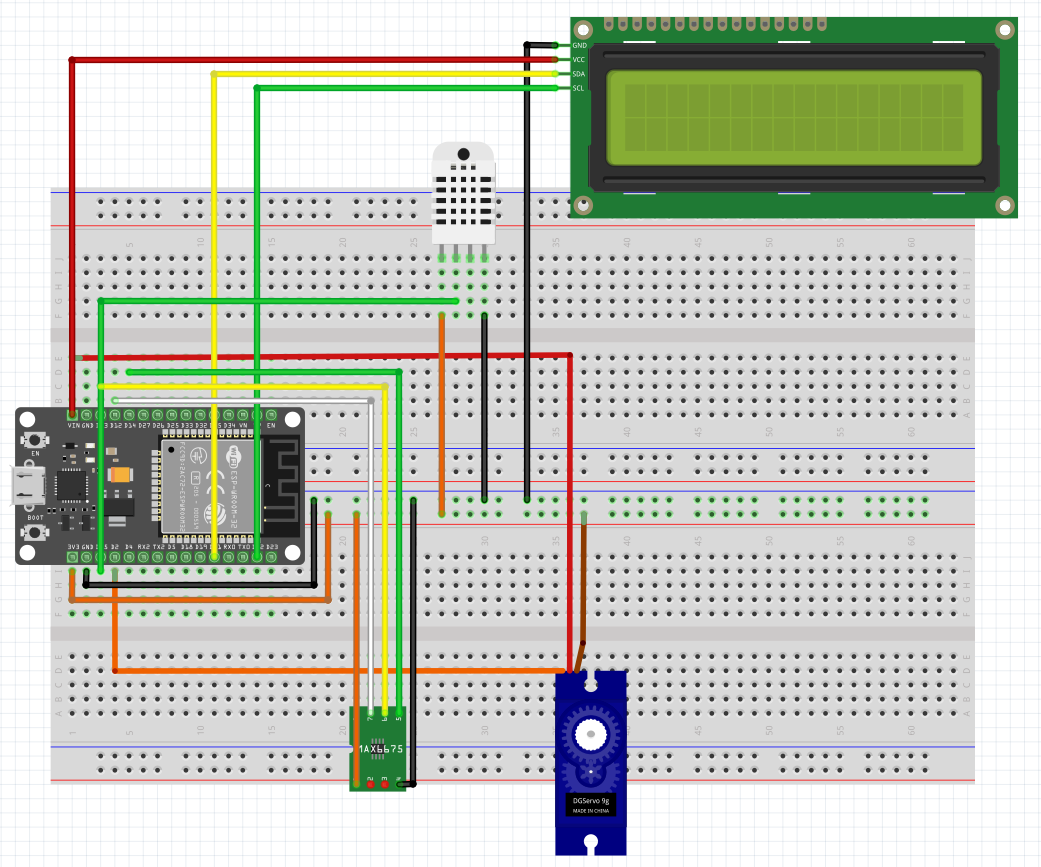
\includegraphics[width=0.8 \textwidth]{fig/fritzing_bredboard_v1.png}
\caption{Wizja elementów sterownika. Opracowanie własne.}
\label{fig:wizja}
\end{figure}
 
 \section{Dalsze kierunki rozwoju}
 W tej części zostaną opisane możliwe kierunki rozwoju sterownika.
 
 Integracja z systemem odzyskiwania ciepła ze spalin.
 Zmiana frameworka z Arduino na Espressif IoT Development Framework - bardziej profesjonalne rozwiązanie, lepsza współpraca z mikrokontrolerem.
 \ldots
 

 \chapter{Charakterystyka metod obsługi pieca} 
 Obsługa w pełni manualna wymaga stałego nadzoru nad przebiegiem spalania. Jest bardzo absorbująca. Łatwo prowadzi do przekroczenia pożądanych temperatur. Pogarsza efektywność procesu spalania, co prowadzi do obniżenia ogólnej sprawności kotła, większego zapotrzebowania na opał, a w konsekwencji znacznie wyższych kosztów ogrzewania.
 
 Obsługa półautomatyczna pozwala na samodzielną pracę urządzenia pomiędzy momentami dokładania paliwa. Można wyróżnić dwie jej odsłony. Mechaniczna, w której głowica termostatyczna połączona jest z mechanizmem dźwigni. Na jej ramieniu znajduje się łańcuszek lub linka. Zaletą jest niski koszt. Elektroniczna, gdzie stosuje się sterownik pokojowy z serwomechanizmem. Koszt tego rozwiązania jest umiarkowany oraz zapewnia szerokie możliwości regulacji, umożliwiając dokonywanie nastaw lokalnie lub zdalnie. 
 
 Najdroższe jak i najbardziej autonomiczne rozwiązanie stanowi obsługa automatyczna, w której kocioł z podajnikiem paliwa pracuje samodzielnie do kilku dni
 
 
 \chapter{Przegląd istniejących rozwiązań} 
 \section{Standardy integracji inteligentnych urządzeń}
 W przypadku internetu rzeczy producenci nie zwracali uwagi na stworzenie otwartych systemów komunikujących się ze sobą urządzeń. W szczególności ograniczone były działania  podejmowane dla umożliwienia doraźnego współdziałania elementów składających się na internet rzeczy pomimo, że organizacje standaryzacyjne zaproponowały wiele protokołów. Żaden z tych standardów nie zdobył na tyle dużej popularności by zdominować pozostałe rozwiązania. Coraz więcej urządzeń podłączanych do internetu udostępnia API, jednak każdy z nich został zaimplementowany z wykorzystaniem innych protokołów i używa innego modelu danych. Zamiast proponować kompletnie nowe standardy, Web of Things wykorzystuje istniejące, dobrze znane standardy webowe.
  
 \section{Sterowniki kominkowe}
 Na Polskim rynku istnieje szeroka gama rozwiązań przeznaczonych do kotłów na paliwo stałe, jednak stosunkowo niewielka ilość sterowników przeznaczonych dla kominków. - tylko z dodatkową przepustnicą co ogranicza możliwość regulacji (powietrze pierwotne i wtórne).
 \subsection{TECH STEROWNIKI}
 Firma TECH ma w swojej aktualnej ofercie \cite{Tech} trzy sterowniki do kominków. Dwa znich są do kominków z płaszczem wodnym. Trzeci \cite{TechSterownik} przeznaczony jest do kominków z dystrybucją gorącego powietrza i mógłby zostać zastosowany przy piecu kominkowym. Czujnik mierzy temperaturę spalin.
 Aby mieć możliwość zdalnego dostępu do sterownika należy skorzystać z jednego z dwóch dodatkowych modułów komunikacyjnych - GSM lub Ethernet. Dostęp jest możliwy jedynie przez stronę producenta lub aplikację mobilną, brak publicznego API.
 Sam moduł Ethernet kosztuje około 500zł \cite{TechEthernetCena}.
 \subsection{EUROSTER}
 Firma EUROSTER ma w swojej aktualnej ofercie \cite{Euroster} tylko jeden seteronik do kominków. Jest on \cite{EurosterSterownik} przeznaczony do współpracy z kominkiem z płaszczem wodnym więc nie może być zastosowany do pieca kominkowego. Nie posiada możliwości zdalnego dostępu. Czujnik mierzy temperaturę wody obiegowej.
 Cena samego sterownika to około 300zł \cite{EurosterSterownikCena}. Dodatkowo należy zakupić przepustnicę.
 \subsection{Kratki}
 Firma Kratki ma w swoje ofercie \cite{Kratki} jeden sterownik do kominków występujący w kilku wersjach różniących się obudową i wielkością dołączonej do zestawu przepustnicy.
 Jest on przeznaczony do współpracy z kominkami każdego rodzaju dlatego może zostać zastosowany do pieca kominkowego. Nie posiada możliwości zdalnego dostępu. Czujnik mierzy temperaturę w pobliżu paleniska. 
 Cena samego sterownika to około 400zł \cite{KratkiSterownik}.
  \subsection{Podsumowanie}
  Tylko jeden z wymienionych producentów pozwala na zdalny dostęp do sterownika, jednak jest on tylko możliwy za pośrednictwem serwerów producenta. Brak publicznego API. Cena tego rozwiązania jest wysoka.
  Tylko jeden z wymienionych sterowników posiada czujnik pozwalający na mierzenie temperatury spalin.
  
  
 \chapter{Opracowanie koncepcji}
 Regulacja dopływu powietrza do komory spalania. Jak dobrać otwarcie przepustnicy? Pomiar temperatury spalin.
 W minimalnej wersji: pomiar temperatury spalin i dobranie otwarcia przepustnicy. Potrzebne tylko mikrokontroler, serwo oraz termopara.
 Dodatki:
 \begin{enumerate}
 \item termometr mierzący temperaturę w pomieszczeniu aby zwiększać moc przy większym zapotrzebowaniu na energię
 \item wyświetlacz przekazujący informacje użytkownikowi
 \item wyjście sterujące wentylatorem wymuszający obieg powietrza do innych pomieszczeń dla lepszej dystrybucji energii
 \item czujnik otwarcia drzwi paleniska aby zmieniać parametry pracy po dołożeniu drewna
 \item zdalny dostęp do sterownika dla ułatwienia obsługi
 \item rtc dla programowania zadań czasowych
 \item połączenie Ethernet, usunięcie niepotrzebnego ruchu WiFi.
 \item zapasowe źródło zasilania, pozwalające na kontrolę pracy pieca w razie zaniku napięcia w sieci
 \item zewnętrzny termometr, automatyka pogodowa
 \item przyciski na sterowniku, do zmiany podstawowych parametrów
 \end{enumerate}  
 
  
 \chapter{Wybór podzespołów}
 \section{Mikrokontroler lub platforma komputerowa}
 Rozważanymi kandydatami na serce sterownika były platformy komputerowe:
 \begin{enumerate}
 \item RaspberryPi
 \item OrangePi
 \end{enumerate}
 oraz mikrokontrolery:
 \begin{enumerate}
 \item Seria Arduino
 \item STM32F103C8T6
 \item ESP8266
 \item ESP32
 \end{enumerate}
 
 Ze względu na koszt jak i rozdzielenie odpowiedzialności zdecydowano się na wybór mikrokontrolera.
 ESP32 - układ SoC, następca ESP8266, wbudowane wi-fi, bluetooth, dwa rdzenie, energooszczędność, stosunkowo niska cena, gotowy moduł pozwalający na wygodne prototypownie.
 
 \section{Wyświetlacz}
 Ze sterownika będą też korzystać osoby o pogorszonym wzroku, dlatego wyświetlacz powinien być duży i kontrastowy.
 Ze względu na to, że wszytki parametry sterownika będą dostępne przez stronę internetową, wybrany został wyświetlacz LCD 2x16 który pozwoli na prezentowanie tylko kilku wybranych parametrów.
 
 \section{Termometr}
 Wybrany układ termometru DHT22 pozwala na pomiar temperatury i wilgotności jednocześnie zapewniając dobrą dokładność odczytów.
 
 \section{Termopara}
 Układ MAX6675 jest jednym ze starszych rozwiązań dostępnych na rynku, a dzięki temu niedrogi i dobrze przetestowany. 

 \section{Układ poruszający przepustnicą} 
 Posiadany piec kominkowy potrzebuje przemieszczania liniowego przepustnicy jednak odpowiednie serwomechanizmy są wciąż drogie i przewyższałyby swoją ceną koszt pozostałych podzespołów całego sterownika.
 Istnieje możliwość zaprojektowania i wydrukowania właściwego adaptera serwomechanizmu, jednak długi czas produkcji oraz testowania wytrzymałości przekraczałby zakres tej pracy.
  Ze względu na niewielką wymaganą precyzję ustawienia przepustnicy oraz zaistniałe opory, wybrano standardowej wielkości, analogowe serwo MG-995, bez adapterów przekształcających na ruch liniowy.
 
 \section{Moduł Ethernet}
 Ponieważ sterownik bez przerwy komunikuje się z Bramą, to aby nie generować smogu elektromagnetycznego zdecydowano na dołączenie dodatkowego modułu komunikacji Ethernet. Wybrany moduł W5500 Lite jest nieznacznie droższy ale za to bardziej kompaktowy niż inne rozwiązania oparte o układ W5500.
 
 \section{Zegar czasu rzeczywistego}
 Pierwotnie planowano wykorzystanie modułu czasu rzeczywistego z podtrzymaniem, jednak ponieważ sterownik przez większość czasu będzie podłączony do internetu skąd może pozyskać aktualną godzinę, zrezygnowano z tego rozwiązania.
 
 \section{Urządzenie wskazujące}
 Pierwszym planowanym rozwiązaniem było wykorzystanie przycisków typu pushbutton. Ponieważ mikrokontroler ESP32 posiada specjalne piny umożliwiające rozpoznawanie dotyku poprzez detekcję zmian pojemności, zdecydowano się zastąpić pushbuttony panelem dotykowym.
 
 \section{Czujnik otwarcia drzwi paleniska}
 Czujnik otwarcia drzwi paleniska pozwoli na wykrywanie momentów dokładania paliwa. W projekcie wykorzystano prosty przełącznik podłączony do pinu cyfrowego mikrokontrolera.
 
 \section{Zasilanie awaryjne}
 Najprostszym z rozważanych rozwiązań było zastosowanie dodatkowego, zewnętrznego modułu typu powerbank, jednak jego wykorzystanie nie dawałoby, żadnej kontroli nad trybem zasilania sterownika. Wybrano płytkę rozszerzeń typu battery shield z dwoma bateriami litowo-jonowymi 18650 o pojemności około 3600mAh każda.
 \section{Rodzaj połączenia czujników zewnętrznych}
 Ze względu na łatwość i pewność połączenia zdecydowano na wybranie standardu złącza 8P8C wykorzystywanego w rożnego rodzaju sprzęcie telekomunikacyjnym i komputerowym. Rozpowszechnione jako złącze do budowy sieci w standardzie Ethernet. 8P8C to złącze o ośmiu miejscach na styk i ośmiu stykach.
 
 
 \chapter{Wykonanie prototypu na płytce stykowej}
 W tym rozdziale opisany został proces prototypowania z wykorzystaniem płytki stykowej.
 Płytka stykowa pozwala na łatwe połączenie elementów tworzonego układu. W pierwszej kolejności podzespoły wpinane są w płytkę, a następnie łączone elektrycznie przy pomocy specjalnych przewodów.
 Pierwszym, elementem sterownika umieszczonym na płytce był mikrokontroler ESP32. Ponieważ może być on zasilany przez port USB nie wymagał więc dodatkowych podłączeń. 
 
 \section{Podłączenie mikrokontrolera oraz LCD}
 Użyty w projekcie wyświetlacz LCD 16x2 posiada dodatkowo konwerter I2C który zmniejsza ilość linii niezbędnych do komunikacji z 16 do 4. Wykorzystana do komunikacji magistrala I2C to szeregowa, dwukierunkowa magistrala która wykorzystuje tylko dwie linie komunikacyjne - Serial Data oraz Serial Clock. Transfer danych może być zainicjowany tylko gdy magistrala nie jest zajęta. Poza liniami transferu danych wyświetlacz potrzebuje także pary linii zasilania - masy oraz 5V.
  
 \section{Podłączenie układu DHT22 - termometr i czujnik wilgotności}
 Moduł DHT22 do komunikacji z mikrokontrolerem wykorzystuje magistralę 1-Wire która wykorzystuje pojedynczą linię komunikacyjną. W zależności od długości przewodów należy wybrać właściwy rezystor podciągający. Mikrokontroler ESP32 posiada wbudowany rezystor podciągający o wartości około 50k Ohmów dlatego jeśli przewody przyłączeniowe nie są długie nie ma potrzeby wykorzystywania dodatkowego rezystora.
 Moduł termometru DHT22 potrzebuje dodatkowo zasilania 3,3V.
 
 \section{Podłączenie układu MAX6675 - termopara}
 Układ MAX6675 wykorzystuje do komunikacji magistralę SPI - 3 linie komunikacyjne: SO - Master Input Slave Output ,CS - Chip Select, SCK - Serial Clock. Do zasilania potrzebne jest napięcie 3,3V.
 
 \section{Podłączenie serwomechanizmu}
 Do podłączenia serwomechanizmu wystarczy jedna linia komunikacyjna przesyłająca sygnał PWM oraz zasilanie 5V.
 
 \section{Podłączenie czujnika otwarcia paleniska}
 Czujnik otwarcia drzwi paleniska w postaci prostego przełącznika został podłączony do pinu cyfrowego mikrokontrolera pojedynczą linią komunikacyjną. Linia ta będzie ustawiana w stan wysoki przy pomocy rezystora podciągającego. Otwarcie drzwi spowoduje zwarcie linii do masy. 
 
  \section{Podłączenie układu W5500 - Ethernet}
 Moduł W5500 wykorzystuje do komunikacji magistralę SPI - 4 linie komunikacyjne: MO - Master Output Slave Input, SO - Master Input Slave Output ,CS - Chip Select, SCK - Serial Clock.
 Podczas podłączania układu napotkano problemy z komunikacją. Konieczna była zmiana wykorzystywanych pinów mikrokontrolera.
 
 \subsection{Okablowanie}
 Podłączenie zewnętrznych czujników do sterownika wykonano z wykorzystaniem skrętki ekranowanej która zapewnia odporność komunikacji na zakłócenia transmisji.
 
 
 \chapter{Napisanie oprogramowania}
 W tym rozdziale opisano proces pisania pierwszej części oprogramowania stanowiącej podstawę komunikacji z modułami sterownika.
 
 \section{Utworzenie projektu}
 Do programowania sterownika wykorzystano środowisko programistyczne CLion wraz z ekosystem PlatformIO.
 CLion to wieloplatformowe zintegrowane środowisko programistyczne (IDE) przeznaczone dla języków C/C++.
 PlatformIO Core jest sercem całego ekosystemu PlatformIO ułatwiającego programowanie mikrokontrolerów. Dostarcza interfejs wiersza poleceń. Jest napisane w Pythonie.
 Projekt oprogramowania sterownika został zainicjalizowany w pustym katalogu poleceniem:
 \begin{lstlisting}
platformio init --ide clion --board esp32doit-devkit-v1 
 \end{lstlisting}
 Definiuje ono z jakiego IDE chcemy skorzystać, oraz jaki mikrokontroler będzie programowany.
 Następnie projekt został otwarty w CLion, gdzie przebiega dalszy proces programowania.
 
 \section{Konfiguracja Projektu}
 W celu konfigurowania projektu należy poddać edycji plik platformio.ini. Daje on przede wszystkim możliwość wybrania frameworka, dodatkowych bibliotek, prędkości komunikacji z mikrokontrolerem przez monitor portu szeregowego oraz parametrów wgrywania oprogramowania.
 
 \section{Szkielet do budowy aplikacji}
 Spośród dwóch dostępnych dla mikrokontrolera ESP32 frameworków ze względu na dużą ilość gotowych bibliotek do komunikacji z modułami zdecydowano się na wykorzystanie platformy programistycznej Arduino.
 Program napisany dla tej platformy musi posiadać plik main w którym są dwie funkcje: setup oraz loop.
 Setup wykonywany jest tylko raz po uruchomieniu mikrokontrolera, natomiast loop wykonuje się w nieskończonej pętli aż do momentu zakończenia pracy.
 
 \section{Dodanie bibliotek i podstawowa komunikacja z urządzeniami}
 Aby sprawdzić poprawność działania prototypu wykonanego na płytce stykowej pisanie oprogramowania rozpoczęto od dodania bibliotek pozwalających na komunikację z urządzeniami. Dla każdego urządzenia stworzono osobny plik .h zawierający deklaracje funkcji oraz plik .cpp zawierający ich definicje.
 W dalszej kolejności zostało opisane użycie poszczególnych bibliotek.
  \subsection{Portal przechwytujący}
 W pierwszej kolejności aby umożliwić łatwą konfigurację połączenia Wi-Fi w sterowniku wykorzystano bibliotekę ESP Acync WiFiManager \cite{WiFiManager} która pozwala na automatyczne tworzenie sieci WiFi i portalu przechwytującego dającego możliwość wybrania i połączenia się z docelową siecią WiFi zapewniającą łączność sterownika z Internetem. 
 Dla utworzenia  WiFi Menagera należy konstruktorowi przekazać dwa obiekty: serwer web oraz server dns. Następnie należy dodać funkcję zwrotną (callback) wykonywaną w momencie utworzenia przez WiFi Manger acces pointa. Aby uruchomić Menager należy wywołać metodę autoConnect przekazując jej jako opcjonalne parametry nazwę acces pointa oraz hasło. Po uruchomieniu Menager próbuje się połączyć z poprzednio zapamiętaną siecią WiFi. Jeśli jej nie odnajdzie, tworzy acces point oraz portal przechwytujący w którym można wybrać inną sieć. Po poprawnym połączeniu na port szeregowy wypisywany jest adres ip sterownika.
 \subsection{Biblioteka dla DHT22}
 Do komunikacji z czujnikiem temperatury i wilgotności wykorzystano bibliotekę DHT sensor library for ESPx \cite{DHTlibrary}. Aby zainicjować działanie biblioteki należy skorzystać z metody setup podając jako parametry numer pinu do którego podłączony jest czujnik oraz model czujnika. Do odczytania pomiarów służą metody getTemperature oraz getHumididity.
 \subsection{Biblioteka dla MAX6675}
 Do komunikacji z termoparą wykorzystano bibliotekę MAX6675 library \cite{MAX6675library}. Aby zainicjować bibliotekę należy skorzystać z konstruktora przekazując jako parametry numery pinów do komunikacji magistralą SPI.
 W celu odczytania temperatury należy skorzystać z metody readCelsius.
 \subsection{Biblioteka dla LCD}
 Do komunikacji z wyświetlaczem LCD z wykorzystaniem magistrali I2C wykorzystano bibliotekę LiquidCrystal PCF8574 \cite{LCDlibrary}. Aby zainicjować bibliotekę należy skorzystać z konstruktora przekazując jako parametr adres wyświetlacza na magistrali. Aby włączyć podświetlenie wyświetlacza należy skorzystać z metody setBacklight. Do wypisywania tekstu na wyświetlaczu służą metody print oraz println.
 \subsection{Biblioteka dla serwomechanizmu}
 Do komunikacji z serwomechanizmem wykorzystano bibliotekę ESP32Servo \cite{Servolibrary}. Aby rozpocząć pracę należy skorzystać z metody attach podając jako argument numer pinu będącego wyjściem sygnałowym. W celu ustawienia mechanizmu na wybraną pozycję należy skorzystać z metody write. Metoda detach służy do przerwania komunikacji z serwomechanizmem.
 \subsection{Biblioteka PID}
 Do sterowania wychyleniem serwa oraz ustalaniem zadanej temperatury w kominie wykorzystano bibliotekę PID \cite{PIDlibrary}. Pozwala ona wykorzystanie regulatora proporcjonalno-całkująco-różniczkującego do utrzymywania wartości wyjściowej na zadanym poziomie.
 Aby zainicjować bibliotekę  należy skorzystać z konstruktora przekazując jako parametr referencje do wartości wejściowej, wyjściowej, zadanej oraz trzy parametry regulatora. Przy pomocy funkcji SetSampleTime należy ustalić jak często regulator ma obliczać wartość wyjściową. Funkcja SetOutputLimits służy do określenia granic parametru wyjściowego, funkcja SetControlDirection służy do określenia kierunku sprzężenia wejścia z wyjściem, funkcja SetMode(AUTOMATIC) uruchamia działanie regulatora.
 \subsection{Biblioteka dla DS18B20}
 Do komunikacji z termometrem Dallas wykorzystano bibliotekę DallasTemperature \cite{dallaslibrary}. Aby zainicjować bibliotekę należy skorzystać z konstruktora przekazując jako parametr referencję do obiektu oneWire. W celu odczytania temperatury nalezy skorzystać z metody requestTemperatures, a następnie getTempCByIndex.
 \subsection{Biblioteka dla W5500}
 Do komunikacji z modułem W5500 wykorzystano bibliotekę Ethernet Library for Arduino \cite{ethernetlibrary}. Aby zainicjować bibliotekę należy użyć metody init podając jako parametr numer pinu Chip Select. Następnie należy skorzystać z metody WizReset wykonującej sekwencję resetowania modułu. W celu rozpoczęcia połączenia Ethernetowego należy użyć metody begin podając jako parametry adres MAC, adres IP, adres DNS, adres bramy oraz maskę.
 \subsection{Biblioteka WebThing}
 Do obsługiwania sterownika jako rzecz webową wykorzystano bibliotekę webthing-arduino \cite{webthinglibrary}. Biblioteka tworzy prosty serwer implementujący Web of Things API.
 Aby zainicjować bibliotekę należy skorzystać z konstruktora przekazując jako parametry nazwę oraz adres IP. Następnie należy utworzyć instancję urządzenia oraz dodać do urządzenia jego właściwości. Aby rozpocząć pracę serwera należy skorzystać z metody begin. Do przekazywania wartości właściwości urządzenia służą metody setValue oraz update.
 
 \section{Zdalne uaktualnianie oprogramowania}
 Mechanizm Over The Air Update pozwala na wgrywanie nowych wersji oprogramowania przez sieć LAN lub Internet (jeśli urządzenie posiada publiczny adres IP). W celu uruchomieniu OTA należy w pliku konfiguracyjnym jako protokół wgrywania wybrać espota, a następnie podać adres urządzenia. Dodatkowo dla zabezpieczenie przed nieuprawnioną zmianą oprogramowania należy ustawić hasło blokujące dostęp.
 
 \section{Odczyt napięć}
 Aby odczytać wartości napięć pinów mikrokontrolera w pierwszej kolejności należy przy pomocy metody pinMode określić numer pinu oraz tryb pracy (INPUT), a następnie skorzystać z metody analogRead.

 
 \chapter{Wykonanie prototypu na płytce uniwersalnej}
 \section{Rozmieszczenie elementów}
 Dla wygodnego połączenia elementów wybrano płytkę uniwersalną o rozmiarach 9cm x 15cm ze standardowym rastrem otworów.
 Na początku na płytce zostały umieszczone największe elementy: bateria z układem zabezpieczającym oraz mikrokontroler. Elementy te zostały połączone z płytką przy pomocy goldpinów. Kolejne elementy rozmieszczano tak aby porty komunikacyjne oraz zasilania znajdowały się na dwóch krawędziach płytki.
  \section{Panel dotykowy}
 Stworzenie i podłączenie panelu dotykowego.
 Trudność w podłączaniu - błędnie nazwane piny ESP32.
 \section{Połączenie elementów}
 Złącza dla goldpinów wszystkich elementów zostały przylutowane do płytki uniwersalnej, a następnie połączone jednożyłowymi przewodami miedzianymi w izolacji. Różne kolory izolacji ułatwiają identyfikację połączeń. Zasilanie do złączy RJ-45 zostało doprowadzone tak aby oba przewody znajdowały się w jednej parze, co pozwala na zmniejszenie ilości generowanych zakłóceń.
 Sprawdzenia poprawności połączeń dokonano przy pomocy miernika uniwersalnego.
 
 
 \section{Web Thing Adapter}
 Wykorzystanie biblioteki WebThingAdapter pozwala na łatwe przekształcenie mikrokontrolera w Rzecz Webową.
 Dodanie dwóch osobnych Rzeczy pozwoli na rozdzieleni funkcji administracyjnych od opcji przeznaczonych dla zwykłego użytkownika.
 
 \section{User Menu}
 Na głównym ekranie wyświetlone są parametry pracy sterownika.
 Proste menu pozwala na zmianę zadanej temperatury w pomieszczeniu.
 
 \section{Logika aplikacji}
 \subsection{Czas rozpalania}
 \subsection{Sygnalizowanie potrzeby dołożenia paliwa}
 \subsection{Zmiana działania po dołożeniu paliwa}
 \subsection{Regulacja pracy wentylatora}
 \subsection{Zamykanie przepustnicy po wypaleniu paliwa}
 
 \section{Dostrajanie parametrów}
 Parametry sterownika zostały dostrojone podczas wykorzystywania sterownika do kontrolowania pracy pieca kominkowego.
 
 
 \chapter{Przetestowanie oprogramowania}
 Głównie testy manualne działającego sprzętu.
 Wykresy w Bramie pokażą możliwość ciągłej pracy.
 Testy jednostkowe logiki aplikacji, najlepiej TDD.
 \section{Testy jednostkowe}
 Testy jednostkowe zostały wykonane z wykorzystaniem Platformio Unit Testing \cite{PIOUnitTesting}. Pozwala na wykonywanie testów na urządzeniu docelowym lub z użyciem platformy Native, wtedy testy są przeprowadzane tylko w środowisku programistycznym.

 
 \chapter{Zintegrowanie z Mozilla Gateway}
 \section{Lokalizacja Bramy Mozilla WebThing}
 Dodanie polskiej wersji językowej do Mozilla Gateway dla zwiększenia dostępności rozwiązania.
 \section{Instalacja Bramy na Raspberry Pi}
 \section{Dodanie urządzeń do Bramy}
 
 \chapter{Przygotowanie instrukcji obsługi}
 Obserwacja - rzadka konieczność dostosowywania parametrów sterownika sprawia, że użytkownicy zapominają o tym jak konfigurować sterownik.
 
 
 \chapter{Efekt końcowy na tle koncepcji}
 Refleksja na temat tego jak wygląda to co zaplanowałem w stosunku tego co udało się uzyskać.
 
 
 \chapter*{Podsumowanie}
 \addcontentsline{toc}{chapter}{Podsumowanie}
 Wnioski, jaką drogę przeszliśmy. Rozdział po rozdziale opisujemy co było wyzwaniem.
 
 
 \chapter*{Dalszy kierunek prac}
 \addcontentsline{toc}{chapter}{Kierunki dalszych prac}
 Jeśli zaczynałbym projekt z moją dzisiejszą wiedzą jak podszedłbym do problemu. Jak dalej rozwijałbym pracę, jakie dalsze tematy zostałyby podjęte. 


% \chapter*{Podsumowanie}

% Nasz wybór (patrz: s.~\pageref{sec:wybor}) miał istotne znaczenie.
% O tym, co było następnie, pisaliśmy w podrozdziale \ref{sec:nastepnie}.
% Konsekwencje\,\ldots

 
  \nocite{*}
% \bibliography{library}
% \bibliographystyle{acm}
 
 \inputencoding{utf8}
 
 \addcontentsline{toc}{chapter}{Książki}
 \printbibliography[title={Książki},type=book]
 
 \addcontentsline{toc}{chapter}{Artykuły}
 \printbibliography[title={Artykuły},type=article]
 
 \addcontentsline{toc}{chapter}{Prace dyplomowe}
 \printbibliography[title={Prace dyplomowe}, type=thesis]
 
 \addcontentsline{toc}{chapter}{Materiały konferencyjne}
 \printbibliography[title={Materiały konferencyjne},type=inproceedings]
 
 \addcontentsline{toc}{chapter}{Pozostałe źródła}
% \printbibliography[title={Pozostałe źródła}, nottype=article, nottype=book, nottype=inproceedings, nottype=thesis]

 

 \end{document}

